% !TeX TXS-program:bibliography = txs:///biber
\documentclass[unknownkeysallowed]{beamer}
\usetheme{UniKlu}
\usepackage[backend=biber,style=apa,sorting=nty, bibencoding=utf8]{biblatex}
\addbibresource{refs.bib}


\usepackage{xcolor}

\title{Collective Self-awareness in Multi-Robot Systems}
\author{Mohammad Rahmani}
\institute{DECIDE Doctoral School}

\begin{document}
\begin{frame}
	\maketitle
\end{frame}

\begin{frame}{Self-awareness (SA) - Overview}
	\begin{itemize}
		\item SA is a concept from psychology/biology which is tried to be implemented in AI. 
		
		\item \textbf{Psychological definition}: Capacity to become object of own attention by perceiving environmental events and correlating them with internal states and memories to improve inference ability  \footnote{\tiny{\fullcite{morin-2006-levels-of-consciousness-and-self-awareness-a-comparison-and-integration-of-various-neurocognitive-views}}}.
		
		\item The purpose of this presentation is to introduce the basic ideas of SA applicable to AI
	\end{itemize}
\end{frame}


\begin{frame}{Exteroceptive and proprioceptive sensors, Actuators}
	\begin{itemize}
		\item Each Intelligent Agent (IA) either biological or artificial is composed of:
			\begin{itemize}
				\item \textbf{Extroceptive sensors}: Sensors to receive data from the world outside
					\begin{itemize}
						\item Human eye
						\item Automatic Vehicle (AV) front Camera
					\end{itemize}
				\item \textbf{Proprioceptive sensors}: To measure internal states
					\begin{itemize}
						\item Human cochlea for balance assessment
						\item AV's speed meter to measure speed
					\end{itemize}
				\item \textbf{Actuators}: To transform aforementioned sensory data to actions.
					\begin{itemize}
						\item Human feet
						\item AV's engine
					\end{itemize}
			\end{itemize}
	\end{itemize}
\end{frame}

%slide 2
\begin{frame}{Inference from contextual data}
	\begin{figure}
		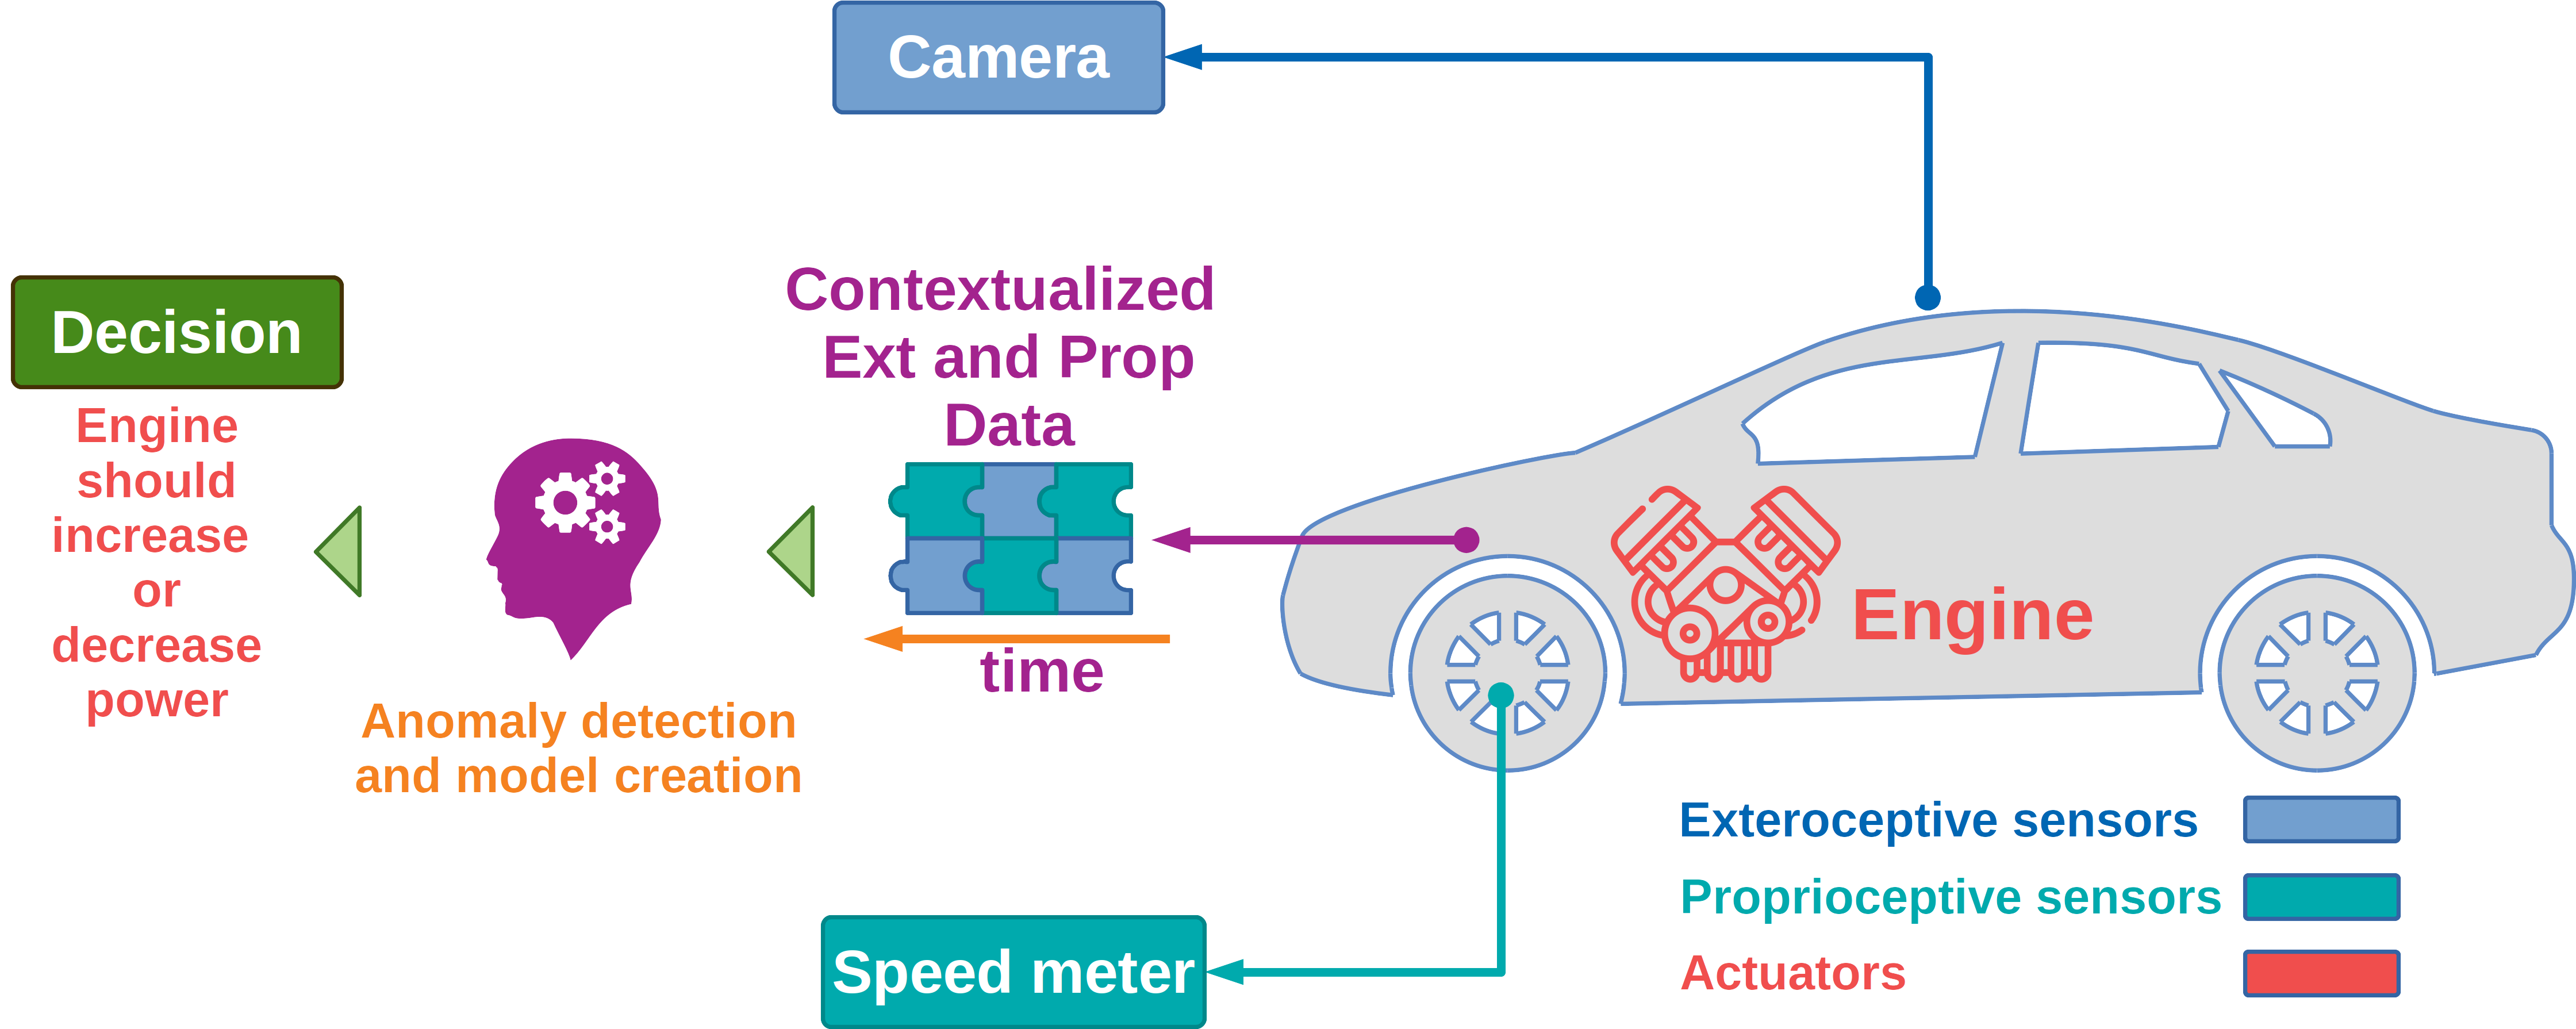
\includegraphics[scale=0.7]{ext-prp-brain.png}
		\caption{Model creation from anomaly}
	\end{figure}
\end{frame}

\begin{frame}{What should be inferred.}
	\begin{itemize}
		\item Sample Contextual data: $v_{t_1}=100kmph$ , $s_{35^{\circ}-20m}$ , $v_{t_2}=60kmph$
		\item What should be inferred?
		\begin{itemize}
			\item \textbf{Causal inference}: Slope $\Rightarrow$ Changes in speed
			\item \textbf{Temporal inference}: Departure with a lower speed from a slope than the arrival $\Rightarrow$ An uphill slope
\item \textbf{Temporal-causal inference} Uphill slope $\Rightarrow$ \textbf{Decision} Engine power increase.
		\end{itemize}
	\end{itemize}
\end{frame}

%slide 3
\begin{frame}{The meaning of SA in AI}
	\begin{itemize}
		\item Temporal-Causal inference from contextualized  \textbf{extroceptive} and \textbf{proprioceptive} data in order to taking better advantage of IA's actuators to achieve its goals.
	\end{itemize}
\end{frame}

%slide 4
\begin{frame}{Mechanism of artificial SA}
	\begin{figure}
		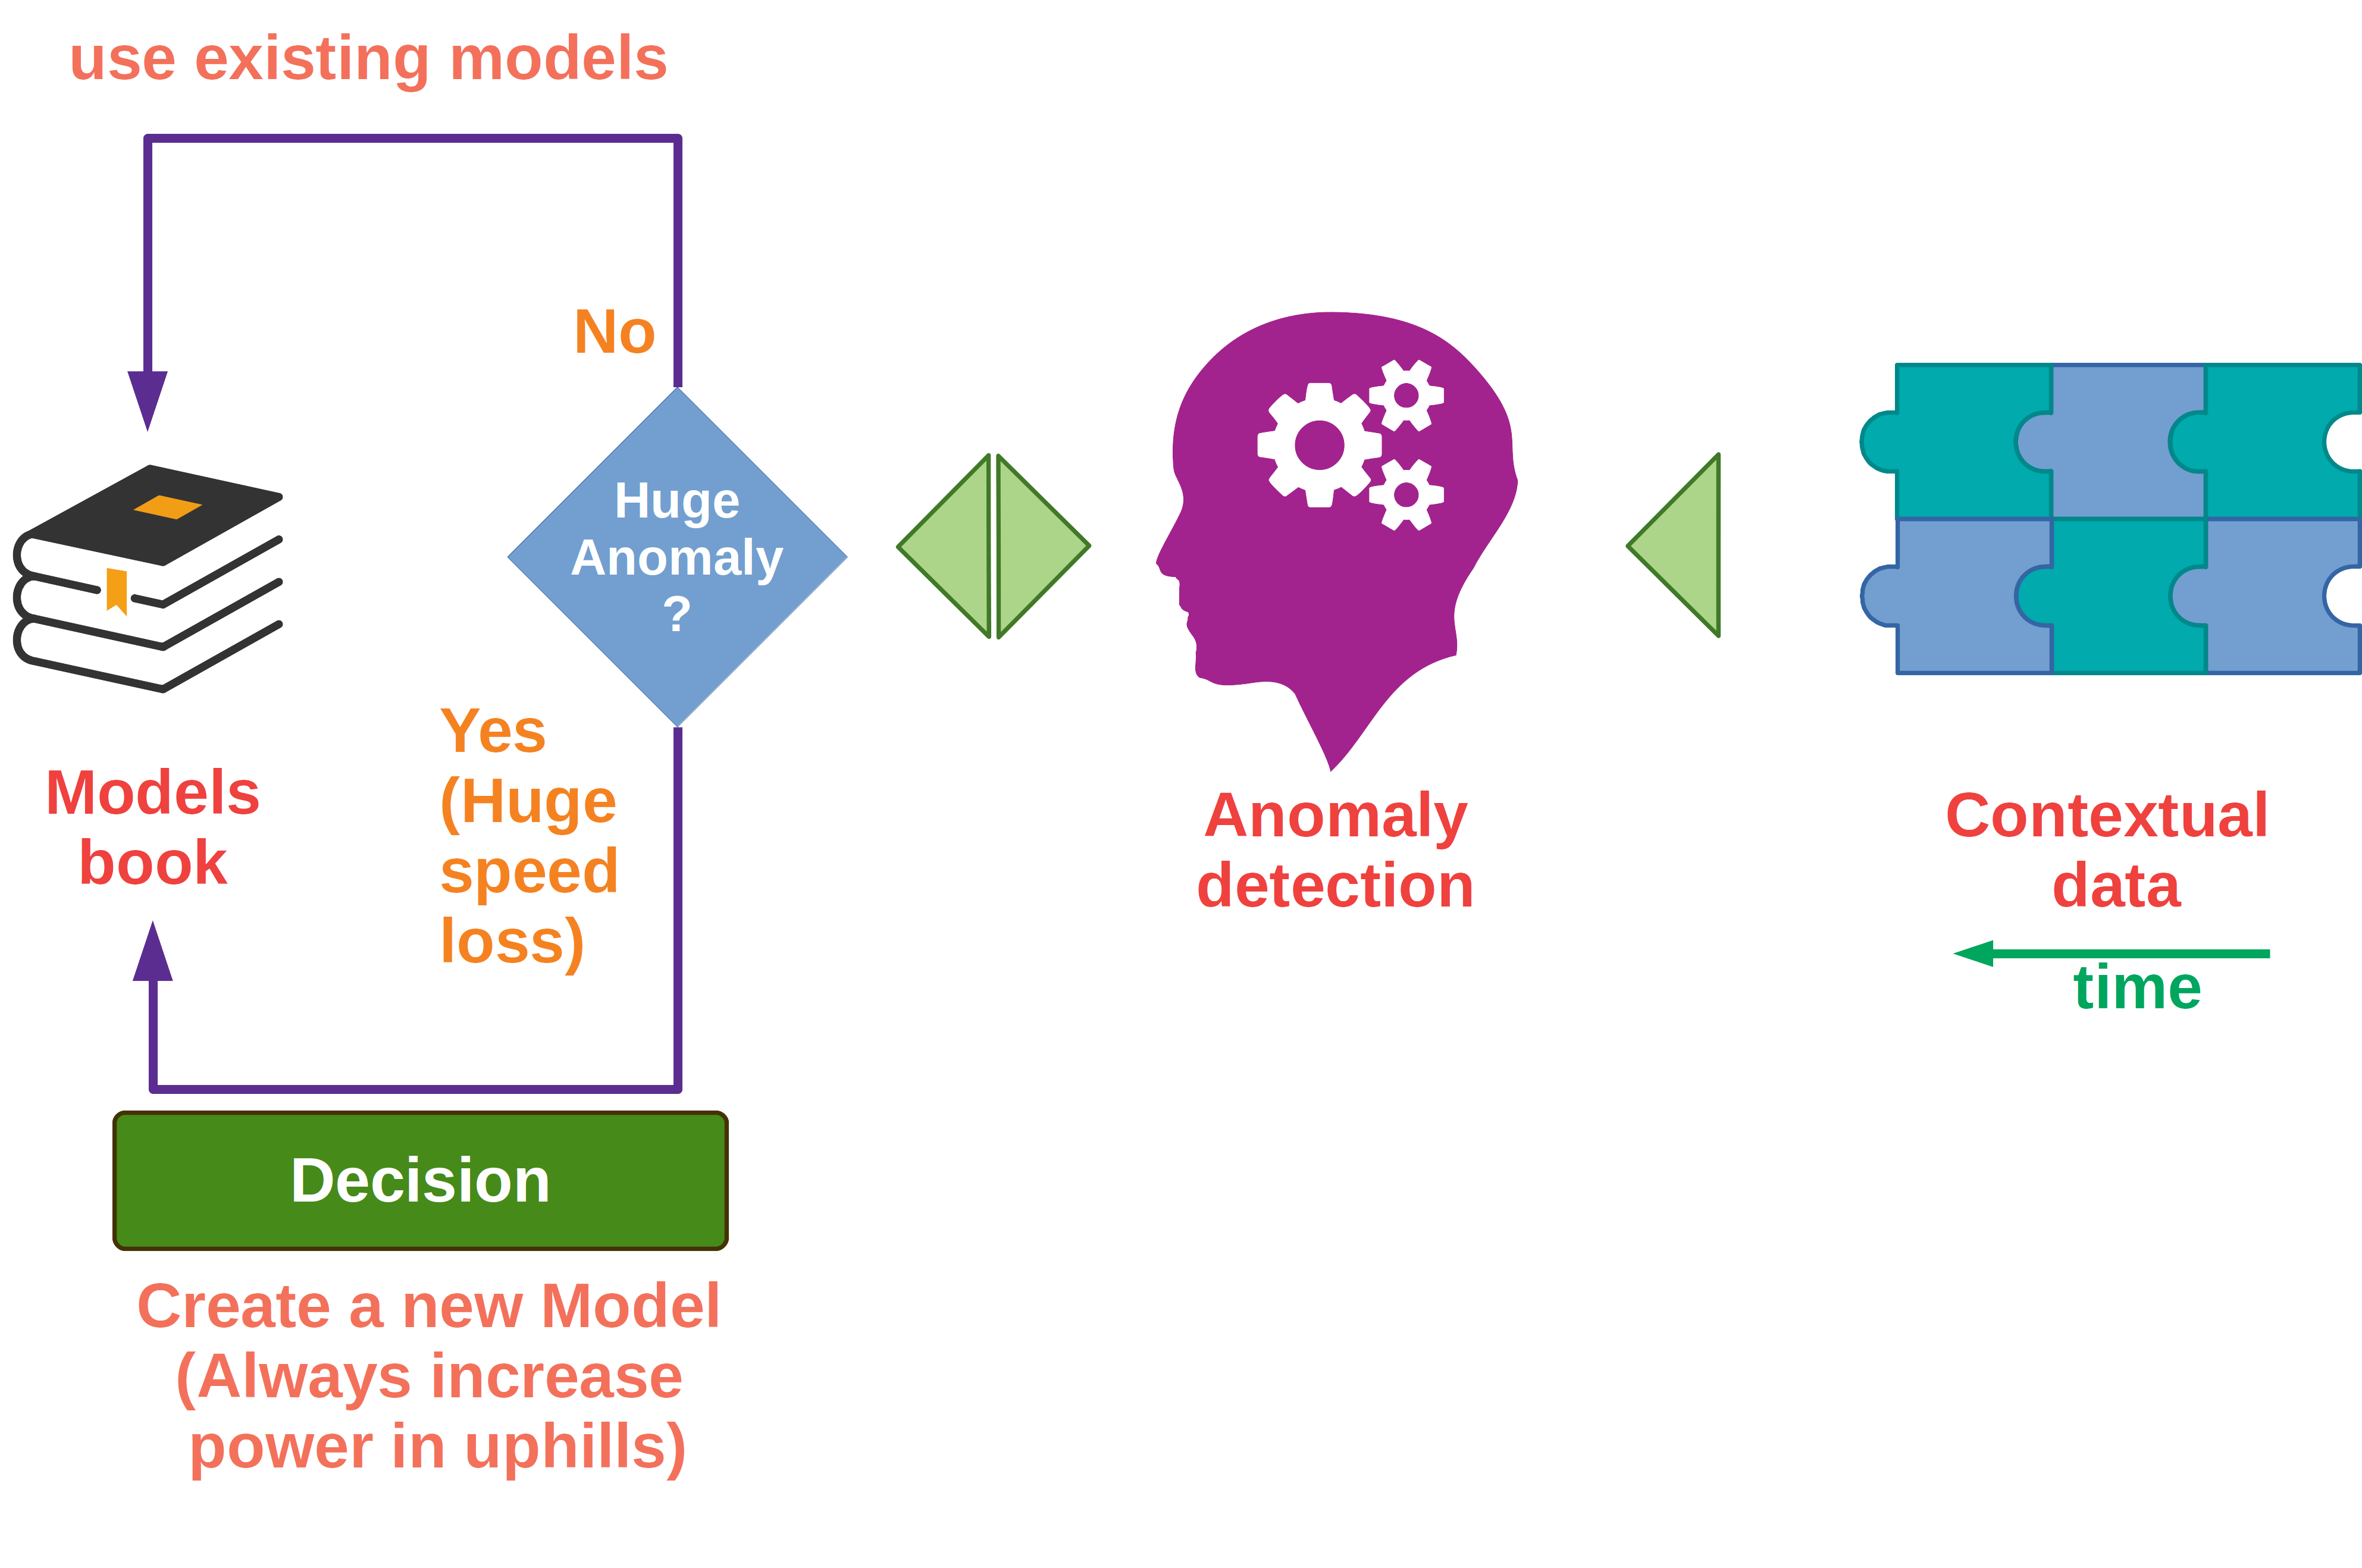
\includegraphics[scale=0.8]{sa-model-creation.png}
		\caption{Model creation from anomaly}
	\end{figure}
\end{frame}

%slide 5
\begin{frame}{Potential benefits of SA for intelligent agents}
	The driving motivation for the transfer of biological SA concepts
	to artificial systems is to improve:
	\begin{itemize}
		\item Autonomy
		\item Robustness
		\item Scalability ( either adding new sensors-actuators or adding new IAs (in case of collective intelligence))
	\end{itemize}
	in an IA \footnote{\fullcite{regazzoni-2020-multi-sensorial-generative-and-descriptive-self-awareness-models-for-autonomous-systems}}.
\end{frame}

\begin{frame}{Tools to implement SA}
	\begin{itemize}
		\item Bayesian Model (BM): To model causality 
		\item Dynamic BM (DBM): To add temporality to causality model 
		\item Coupled DBM (To model dependence between Extroceptive and Proproceptive events)
		\item Generalized filtering (A non-linear space state Bayesian filtering) (To predict future state of an IA)
	\end{itemize}
\end{frame}

\begin{frame}{Collective Self-awareness (CA)}
	\begin{itemize}
		\item When \textbf{proprioceptive} data of one agent turns to be the \textbf{extroceptive} data of the other then we face CA (\textbf{\cite{regazzoni-2020-multi-sensorial-generative-and-descriptive-self-awareness-models-for-autonomous-systems}}).
		\item In other words: Communication among other IAs can be interpreted as exteroceptive data to each IA.
	\end{itemize}
\end{frame}

\begin{frame}{CA examples in biology}
	\textbf{Biological Example}: Ants use pheromone samples left by other ants to locate the food.  \footnote{\tiny{\fullcite{mitchell-2005-self-awareness-and-control-in-decentralized-systems}}}
	\begin{itemize}
		\item Bee colony
		\item Ant colony
		\item human immune system
	\end{itemize}
	\textbf{Particularities}:
	\begin{itemize}
		\item No individual agent shares the whole sensory data it perceives. Instead, it transmit signs to others so that they can make decision on their own. In other words:
		\begin{itemize}
			\item Information is decentralized
			\item Control is decentralized (i.e. each agents acts based on its own “rules”), but a group behavior emerges)
		\end{itemize} 
	\end{itemize}
\end{frame}

\begin{frame}{Artificial CA - Switching between different data forms}
	\begin{itemize}
		\item \textbf{AI Example}: Two AVs following each other. 
		\begin{itemize}
			\item The leader use its camera to navigate.
			\item The follower uses the position and steering data of the leader.
			\item If abnormality occurs in leader's camera data (optical flow) and the leader stops, the follower builds a model using (position,steering) data to imitate the same behavior to stop
			 \footnote{\tiny{\fullcite{kanapram-2020-collective-awareness-for-abnormality-detection-in-connected-autonomous-vehicles}}} \textbf{\cite{regazzoni-2020-multi-sensorial-generative-and-descriptive-self-awareness-models-for-autonomous-systems,kanapram-2019-self-awareness-in-intelligent-vehicles-experience-based-abnormality-detection}}. 
			 \begin{itemize}
			 	\item \textbf{Advantage} The size of (position,steering) data is hugely less than optical follow.
			 	\item \textbf{Popular modeling tool}: Switching DBNs
			 	\item \textbf{Application}: Collective collision avoidance in large numbers of vehicles.
			 \end{itemize}
		\end{itemize}
		
	\end{itemize}
\end{frame}

\begin{frame}{Semantic segmentation in CA}
	\begin{itemize}
		\item Decomposing (making discreet) the data related to a behavior(word) to several sub-behaviors (classes/letters)
	\end{itemize}
	The \textbf{overtaking} behavior/word(a sequence of IDs) in a vehicle is composed of the three sub-behavior/letters(class IDs)
	\begin{itemize}
		\item (position, steering) data related to increasing speed
		\item (position, steering) data related to turning left
		\item (position, steering) data related to turning right
	\end{itemize}
	As in previous slides application of \textbf{contextual data} was introduced, in this slide application of \textbf{contextual semantic} is introduced. It is better known as \textbf{Semantic awareness} (\textbf{\cite{regazzoni-2020-multi-sensorial-generative-and-descriptive-self-awareness-models-for-autonomous-systems}}).
\end{frame}

\begin{frame}{Semantic awareness benefits in CA}
	\begin{itemize}
		\item Transmission of a single word composed of letters instead of the whole data related to (position, steering) since 
		\begin{itemize}
			\item The data is even more simple
			\item It is possible to compose new states and predict future states according to their composing letters to make better decisions without reviewing the whole data.
		\end{itemize}
	\end{itemize}
\end{frame}

\begin{frame}{Tools to implement CA}
	\begin{itemize}
		\item  \textbf{To generate discreet States}: Growing Neural Gas (GNG) for clustering (Sub-behavior/letters/classes) \footnote{\tiny{\fullcite{fritzke-1995-a-growing-neural-gas-network-learns-topologies}}}
		\item \textbf{To predict future states}: Markov Jump Particle Filter (MJPF)  to predict and estimate discrete future states and to detect deviations from the normal model (By establishing DBNs between current and future states)\footnote{\tiny{\fullcite{baydoun-2018-learning-switching-models-for-abnormality-detection-for-autonomous-driving}}} (\textbf{\cite{kanapram-2019-self-awareness-in-intelligent-vehicles-experience-based-abnormality-detection}}).
	\end{itemize}
\end{frame}

\begin{frame}{CA benefits}
	\begin{itemize}
		\item Improves scalability
		\item Reduces computational complexity through local-symbolic interaction
		\item Addresses heterogeneity by creating semantic fields
	\end{itemize}
\end{frame}

\begin{frame}{CA application}
	\textbf{Examples}:
	\begin{itemize}
		\item Agent collision avoidance  \footnote{\tiny{\fullcite{selvaggio-2017-towards-a-self-collision-aware-teleoperation-framework-for-compound-robots}}}
		\item Traffic jam avoidance \footnote{\tiny{\fullcite{qing-2107-real-time-road-traffic-awareness-model-based-on-optimal-multi-channel-self-organized-time-division-multiple-access-algorithm}}}
		\item Collective incident locating \footnote{\tiny{\fullcite{kosak-2019-multipotent-systems-combining-planning-self-organization-and-reconfiguration-in-modular-robot-ensembles}}}
	\end{itemize}
\end{frame}

\begin{frame}{First plans for the PhD}         
	\begin{itemize}
		\item Study the concept of self-awareness, in particular collective SA in MRS
		\item Investigate semantic interaction and semantic-awareness among IAs (what and when to communicate and how to integrate received data in model creation)
		\item Deploy and evaluate concepts in MRS
	\end{itemize}
\end{frame}

\begin{frame}{Some links}
	\begin{itemize}
		\item \textbf{IEEE Forthcoming event}: \textcolor{blue}{\url{https://proceedingsoftheieee.ieee.org/view-recent-issues/july-2020/}}
		\item  \textbf{June 22, presentation}: \textcolor{blue}{\url{https://github.com/donkarlo/mrs-self-awareness/blob/master/docs/decide/june-22/decide-june-22.pdf}}
		\item  \textbf{July 6, presentation}: \textcolor{blue}{\url{https://github.com/donkarlo/mrs-self-awareness/blob/master/docs/decide/july-half-1/decide-july-1st-half.pdf}}
		\item  \textbf{If you like to contribute in my informal MRS SA literature review:}: \textcolor{blue}{\url{https://github.com/donkarlo/mrs-self-awareness/blob/master/docs/decide/july-half-1/decide-july-1st-half.tex}}
	\end{itemize}
\end{frame}

\begin{frame}{Appendix}
	\begin{itemize}
		\item \textbf{Appendix A}: Essential requirements
		\item \textbf{Appendix B}: Levels and Aspects of SA
		\item \textbf{Appendix C}: Damasio Model
	\end{itemize}
\end{frame}

\begin{frame}{Appendix A: Essential requirements}

\end{frame}

\begin{frame}{SA IA Essential requirements}
	See \textbf{
	\cite{regazzoni-2020-multi-sensorial-generative-and-descriptive-self-awareness-models-for-autonomous-systems}}
	\begin{itemize}
		\item \textbf{Initialization}: Initial knowledge from which an agent starts building its own memories (Training phase. \emph{Techniques}: Random walk, Driving an autonomous vehicle a few times human agent. etc). \textbf{Biology}: Implemented into genes.
		\item \textbf{Memorization}: Capability to store and retain information \textbf{Biology}: Brain's capability to fire group memory related neurons in case of facing familiar patterns of stimuli. 
		\item \textbf{Inference}: Ability to predict own future states \textbf{Biology}: See "Predictive coding theory" in \textbf{\cite{seth-2013-interoceptive-inference-emotion-and-the-embodied-self}}
	\end{itemize}
\end{frame}

\begin{frame}{SA IA Essential requirements 2}
	\begin{itemize}
		\item \textbf{Anomaly detection}: Capability to recognize observations which don't match episodes of memory. \textbf{Biology}: Brains ability to send it's predictions to low-level sensory regions to test them against existing memories.
		\item \textbf{Model creation}: Capability of generating models that encode previous experiences for future predictions. \textbf{Biology}: In brain, internal models get adjusted so that the predicting error gets suppressed \textbf{\cite{friston-2010-the-free-energy-principle-a-unified-brain-theory}}.
	\end{itemize}
\end{frame}

\begin{frame}{SA IA Essential requirements 3}
	\begin{itemize}
	\item \textbf{Decision-making influence}: The ability to generate signals that can be employed by the agent’s control system such that its actions are self-monitored dynamically. \textbf{Biology}: Muscles move based on commands from the brain \textbf{\cite{rizzolatti-1996-premotor-cortex-and-the-recognition-of-motor-actions}}. Nerve cells in the spinal cord, called motor neurons, enable to convey and evaluate the brain’s commands to the muscles.
	\end{itemize}
\end{frame}



\begin{frame}{Appendix B: Levels and Aspects of SA}

\end{frame}

\begin{frame}{SA - Levels}
	See \textbf{\cite{lewis-2017-towards-a-framework-for-the-levels-and-aspects-of-self-aware-computing-systems}} - Ordered from basic to advanced
	\begin{itemize}
		\item \textbf{Ecological self} The most basic, referring the ability of an agent to react to an external stimuli. \textbf{I feel, therefore I exist.}
		
		\item \textbf{Interpersonal self} Awareness of external interaction such that limited adaptation to performance of basic homeostatic tasks is achieved.\textbf{I can change the environment, therefore I exist.}
		
		\item \textbf{Extended self}  Permit reflection of interactions over time. The organism is aware of the existence of past and future. \textbf{I feel the course of time, therefore I exist.}
		
		\item \textbf{Conceptual self}: The capability of constructing and reasoning
		about an abstract symbolic representation of itself (AI's goal). \textbf{And finally, I think therefore I exist.}
	\end{itemize}
\end{frame}

\begin{frame}{SA - Aspects}
	See \textbf{\cite{lewis-2017-towards-a-framework-for-the-levels-and-aspects-of-self-aware-computing-systems}}
	\begin{itemize}
	\item \textbf{Identity Awareness}: The ability to recognize and model the identity of agents.
	\item \textbf{State Awareness}: The ability to model and recognize the states of oneself, the world or other entities within it
	\item \textbf{Time Awareness}: The knowledge of past or potential future basic stimuli
	\item \textbf{Interaction Awareness}: The ability to taking into account casual patterns of
	interactions between entities.
	\end{itemize}
\end{frame}

\begin{frame}{SA - Aspects (2)}
	See \textbf{\cite{lewis-2017-towards-a-framework-for-the-levels-and-aspects-of-self-aware-computing-systems}}
	\begin{itemize}
	\item \textbf{Behavior Awareness}: The ability to model the internal behavior of the system
	or behavior of external entities.
	\item \textbf{Goal Awareness}: the ability to conceptualize the internal factors that drive the behavior, such as a system’s goals, objectives, and constraints.
	\item \textbf{Belief Awareness}: Things believed to be true by a system which do \textbf{NOT} need to capture the notion of time.
	\item \textbf{Expectation Awareness}: Combines belief awareness and time awareness, to form models that express what the system or others believe about how the world will unfold over time
	\end{itemize}
\end{frame}

\begin{frame}{Appendix C: Damasio Model}
	
\end{frame}

\begin{frame}{Are there biological models?}
	\begin{itemize}
		\item Damasio \textbf{(\cite{damasio-1999-the-feeling-of-what-happens-body-and-emotion-in-the-making-of-consciousness})}
		\item Haykin \textbf{(\cite{haykin-2012-cognitive-dynamic-systems-perception-action-cycle-radar-and-radio})}
		\item Friston \textbf{(\cite{friston-2010-the-free-energy-principle-a-unified-brain-theory})}
	\end{itemize}
\end{frame}

\begin{frame}{SA - Damasio is a base}
	\begin{itemize}
		\item \textbf{Damasio} presents an architecture for self-awareness but doesn't present a computational model.
		\item \textbf{Haykin} and \textbf{Friston} have to some extent adopted Damasio's architecture to build their computational models to explain observation of an external stimuli leads to decision making. 
	\end{itemize}
\end{frame}

\begin{frame}{Damasio SA}
	\begin{itemize}
		\item Lets divide observations of an agent to \textbf{exteroceptive}
		and \textbf{proprioceptive} observations.
	\end{itemize}
	\begin{figure}
		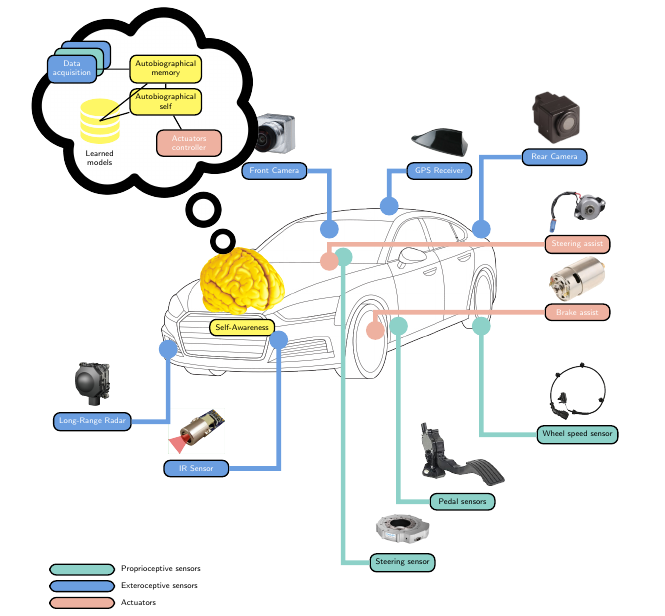
\includegraphics[scale=0.3]{regazzoni-2020-multi-sensorial-generative-and-descriptive-self-awareness-models-for-autonomous-systems-fig-1.png}
		\caption{See \cite{regazzoni-2020-multi-sensorial-generative-and-descriptive-self-awareness-models-for-autonomous-systems}}
	\end{figure}
\end{frame}

\begin{frame}{Damasio - Dispositional units}
	\begin{itemize}
	\item Lets make the contextually put together proprioceptive and extroceptive data over the course of time in two ways:
	\begin{itemize}
		\item Passive: An extroceptive piece of data is surrounded by two proprioceptive pieces of data
		\item Active: A proprioceptive piece of data is surrounded by two extroceptive piece of data 
	\end{itemize}
	\end{itemize}
	\begin{figure}
	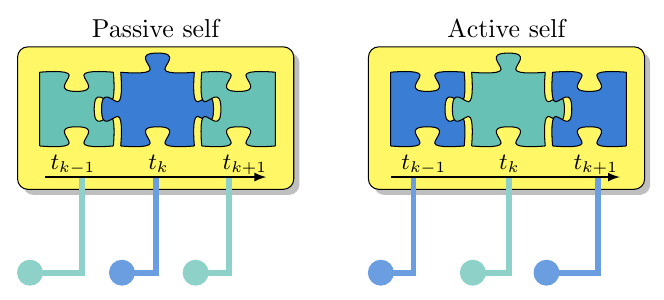
\includegraphics[scale=0.3]{regazzoni-2020-multi-sensorial-generative-and-descriptive-self-awareness-models-for-autonomous-systems-fig-2.png}
	\caption{See \cite{regazzoni-2020-multi-sensorial-generative-and-descriptive-self-awareness-models-for-autonomous-systems}}
	\end{figure}
\end{frame}

\begin{frame}{Damasio - HDU}
	\textbf{Hierarchical Dispositional Units (HDU)}
	\begin{itemize}
	\item To extract casual-temporal inferences, similar to brain, dispositionl units are contextually placed in one another in a hierarchy.
	\end{itemize}
	\begin{figure}
	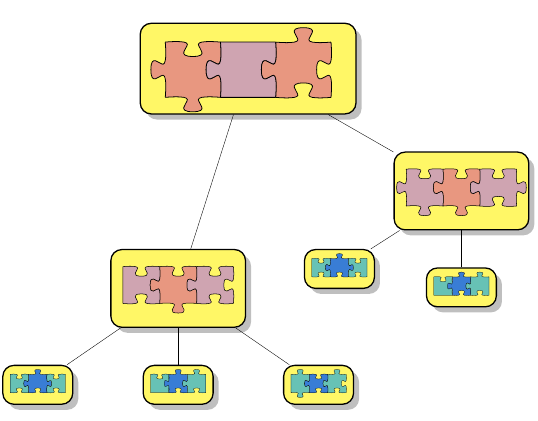
\includegraphics[scale=0.3]{regazzoni-2020-multi-sensorial-generative-and-descriptive-self-awareness-models-for-autonomous-systems-fig-3.png}
	\caption{See \cite{regazzoni-2020-multi-sensorial-generative-and-descriptive-self-awareness-models-for-autonomous-systems}}
	\end{figure}
\end{frame}

\begin{frame}{Damasio - AM}
	\textbf{Autobiographical Memory (AM)}
	\begin{itemize}
	\item Each set of dispositional units which contribute to building an experience is stored as an episode
	\item The collection of all episode forms the architecture of memory in the form a book which each page presents an episode. 
	\end{itemize}
\end{frame}

\begin{frame}{Damasio - AM}
	\begin{figure}
	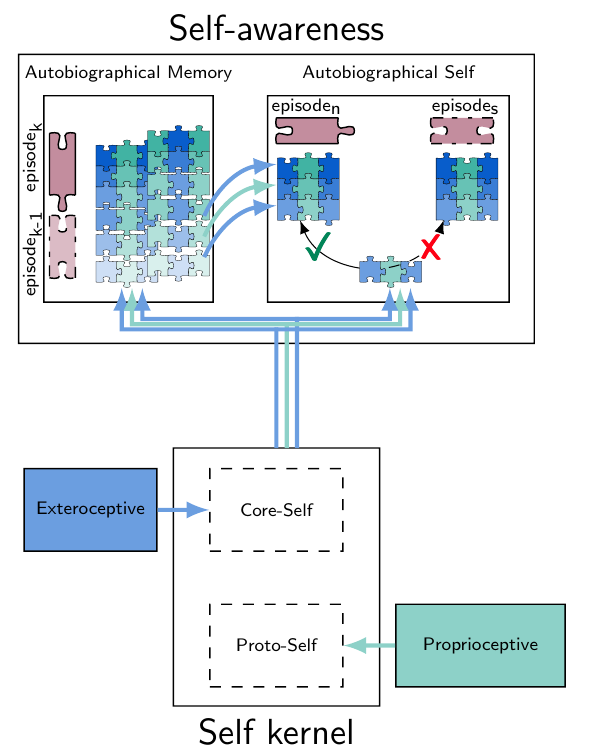
\includegraphics[scale=0.3]{regazzoni-2020-multi-sensorial-generative-and-descriptive-self-awareness-models-for-autonomous-systems-fig-4.png}
	\caption{See \cite{regazzoni-2020-multi-sensorial-generative-and-descriptive-self-awareness-models-for-autonomous-systems}}
	\end{figure}
\end{frame}

\begin{frame}{Damasio - Abnormality}
	\begin{itemize}
	\item Lets open the system's memory to observation through the time.
	\item Try to find a match for the set of observations in all AM pages with some acceptable noise tolerance (Most models use Hellinger metric to measure the distance between model's prediction and the set of observations)
	\begin{itemize}
	\item If there is a prediction(model/episode in AM) that falls bellow the tolerance for that set of observations then activate actuators as the models says. 
	\item If none of the predictions doesn't fall bellow the tolerance then its time to add a new episode (i.e page) to AM.
	\end{itemize} 
	\end{itemize}
	So another definition of self awareness is:
	\begin{itemize}
	\item Learning from large abnormalities
	\end{itemize}	
\end{frame}

\begin{frame}{Damasio - Abnormality}
	\begin{figure}
	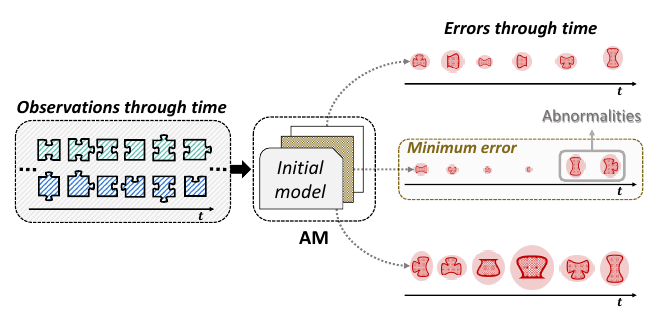
\includegraphics[scale=0.3]{regazzoni-2020-multi-sensorial-generative-and-descriptive-self-awareness-models-for-autonomous-systems-fig-8.png}
	\caption{See \cite{regazzoni-2020-multi-sensorial-generative-and-descriptive-self-awareness-models-for-autonomous-systems}}
	\end{figure}
\end{frame}

\begin{frame}[allowframebreaks]{References}
	\printbibliography
\end{frame}
\end{document}
